\section{Introduction}
\label{sec:introduction}

Recent advances in robotic systems have improved autonomy in perception, manipulation, and planning, yet robots still fail in real-world environments due to perception errors, action execution failures, partial observability, and dynamic changes~\cite{kaipa2016addressing,kaelbling1998planning,kurniawati2016online}. These failures often arise because the robot must select actions from an incomplete or ambiguous estimate of the current world state. In tasks such as tomato harvesting and waste sorting, uncertainty about object states or categories may remain even after sensing, making human feedback a useful source of task-relevant information.

Existing ways of incorporating humans into robot autonomy remain limited. Continuous-supervision and human-on-the-loop systems rely on operators to monitor execution and detect failures~\cite{goodrich2008human,dragan2013legibility,scharre2015introduction,nahavandi2017trusted}, which can increase workload and fatigue~\cite{chen2014human,endsley2018automation,wong2017workload}. Failure-triggered systems reduce monitoring but ask only after errors occur, while fixed or uncertainty-threshold query systems can ask too often~\cite{knowno2023,liang2024introspective,mullen2025lbap}. These approaches leave two coupled questions unresolved: \textit{when} should the robot ask a human, and \textit{what} should it ask?

We trigger human feedback from the robot's belief update rather than treating it as continuous supervision or failure recovery. After each action, the robot compares the observation with possible transition outcomes encoded in its symbolic belief. If multiple task-relevant successor states remain plausible, the system estimates uncertainty using entropy and asks about the symbolic hypothesis expected to reduce the ambiguity. This follows the broader goal of selective assistance, where robots request human input only when it is useful~\cite{sadigh2017active,baraglia2017efficient,leusmann2023understanding}.

This paper proposes a knowledge-based belief-space planning framework for proactive human querying. The robot maintains a symbolic knowledge base~\cite{davis1993knowledge} with STRIPS-style state and action structure~\cite{fikes1971strips}, while online decision making is performed using a POMDP formulation and POMCP-based planning~\cite{kaelbling1998planning,silver2010monte}. Instead of committing uncertain perceptual outputs as deterministic facts, the robot maintains a particle belief over symbolic possible worlds. After each observation, the system updates the belief over reachable frontier states, computes entropy-based confidence, and either commits the most likely state to the knowledge base or asks the human a targeted question before replanning.

\begin{figure}[t]
    \centering
    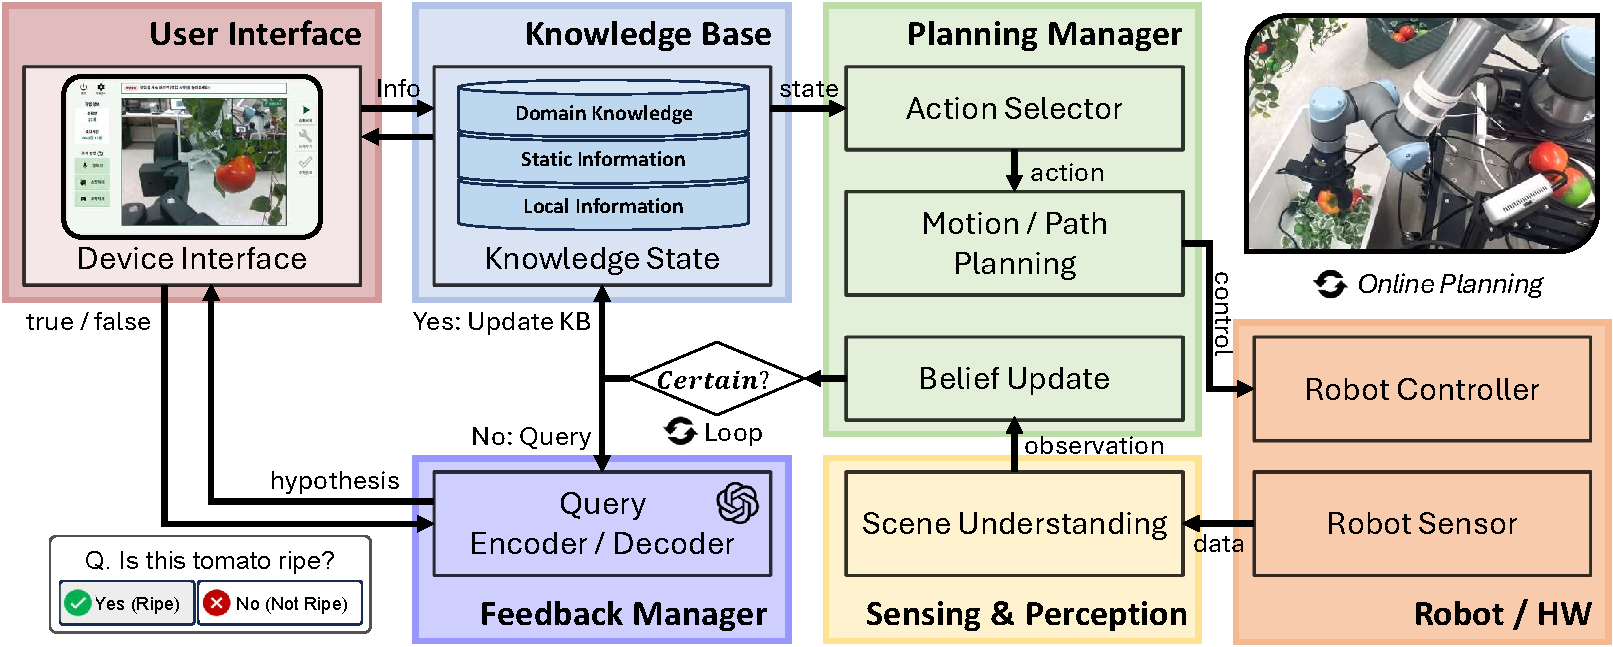
\includegraphics[width=0.95\linewidth]{figures/fig_dataflow.pdf}
    \caption{System architecture and data flow of the proposed framework. The knowledge base stores committed symbolic information, the planning manager maintains and updates the frontier belief, the sensing and perception module provides observations, and the feedback manager queries the user only when belief confidence is insufficient for knowledge-base commitment.}
    \label{fig:overview}
\end{figure}

The framework differs from continuous supervision, failure-triggered intervention, always-query policies, and action-level query systems: the user is not asked to monitor every decision or choose robot actions, but instead answers targeted questions about uncertain symbolic state facts.

We evaluate the framework in waste sorting and tomato harvesting. The main evaluation compares system performance under different confidence thresholds and query policies, while a compact user study analysis examines whether state-level querying changes workload and situation-awareness measures.

The contributions and findings of this paper are:
\begin{itemize}[leftmargin=*]
    \item We formulate human querying as belief refinement in a symbolic planning system: observations update an action-conditioned frontier belief, entropy-normalized confidence determines whether the state can be committed, and queries are selected by expected posterior entropy.
    \item We present an integrated architecture connecting a structured knowledge base, POMCP-style online planning, sensing and perception, feedback management, and knowledge-base commitment.
    \item We show that the confidence threshold $\tau$ controls a sharp autonomy-interaction trade-off, with high task success emerging once the belief is sufficiently constrained by selective feedback.
    \item We compare no-query, random-query, always-query, and proposed query policies to isolate the value of belief-triggered, hypothesis-level querying; user-study results are included as a secondary analysis of interaction burden.
\end{itemize}
